\documentclass{article}
\usepackage{graphicx} % Required for inserting images
\usepackage{amsmath}
\title{Threat hunting principles \\
}
\usepackage{array}
\author{Olof Magnusson}
\date{\today}
\begin{document}
	
	\maketitle
	
	\section*{What question are we trying to answer?}
Threat hunting depends on certain objectives that needs to be addressed. This essentially involves attempts to understand the threat actors objective, the cyber-terrain in which they operate and to identify how we can get closer to those objectives using well-defined searches in different SIEM-platforms. Framing these question in detail will define each scope of a hunt. 



	\section*{Which data do you need for answering the question?}
	It is important to identify what type of data are required for each threat hunting exercise. There are certain circumstances where we might want to specify certain directories in which known bad actors operates and consequently checking for suspicious parent-child process relationships. This type of data can be identified using frameworks like \texttt{MITRE}, where the objectives are stated clearly and their actions can be developed into search terms to be executed in SIEM-platforms. You can begin your analysis using the \texttt{general\_queries} program located in the root directory to identify potential points of communication.
    
	\section*{How do you extract and validate that data?}
	Now that we have extracted search terms - we need to execute it into practice. This can be done using a variety of platforms such as \texttt{Microsoft Defender}, \texttt{Elastic} or \texttt{QRadar} depending on the objective of the threat actor. From the data, we can potentially identify things that are legitimate, unknown, bad or interesting. Furthermore, the findings can then be extracted using \textit{csv} or similiar to visualise the data of the hunt.
	\section*{What does the data tells you?}
	Looking into the collected data to figure out what belongs and what does not belong becomes an important point in this stage of the hunt. Framing questions like: How often does this process runs in this environment or why does this process only occurs at domain controllers aids the analyst to look into the data in several different viewpoints.
	
	\section*{Conclude the threat hunting exercise}
	The conclusion is done by writing a small technical report about the steps you took to facilitate the search terms and what type of findings you identified. This is done to validate the soundness of the threat hunting exercise and to provide room for improvement opportunities. As indicated, the data from the findings can be connected using the STIX framework in Figure \ref{test} to identify relationships.
		
		\begin{figure}[!htb]
			\centering
			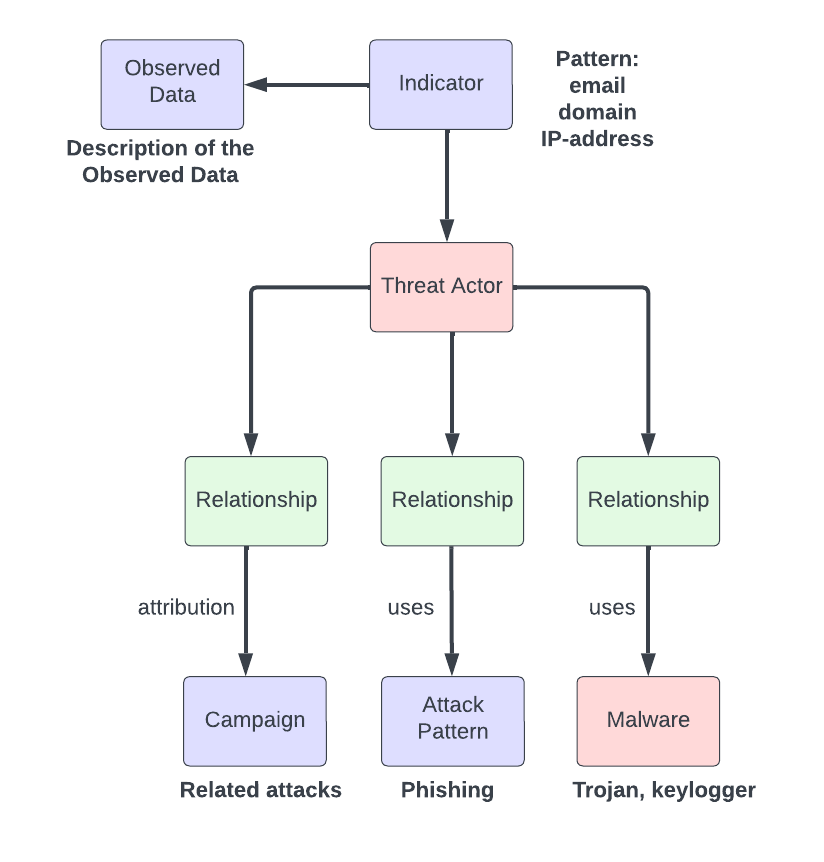
\includegraphics[width=\linewidth]{stix-test.png}
			\caption{STIX-framework}
			\label{test}
		\end{figure}
	
	
\end{document}


